\ylDisplay{Konn} % Ülesande nimi
{Taavi Pungas} % Autor
{lahtine} % Voor
{2010} % Aasta
{G 9} % Ülesande nr.
{9} % Raskustase
{
% Teema: Staatika
\ifStatement
\begin{wrapfigure}{r}{0.35\textwidth}
	\vspace{-1.8ex}
	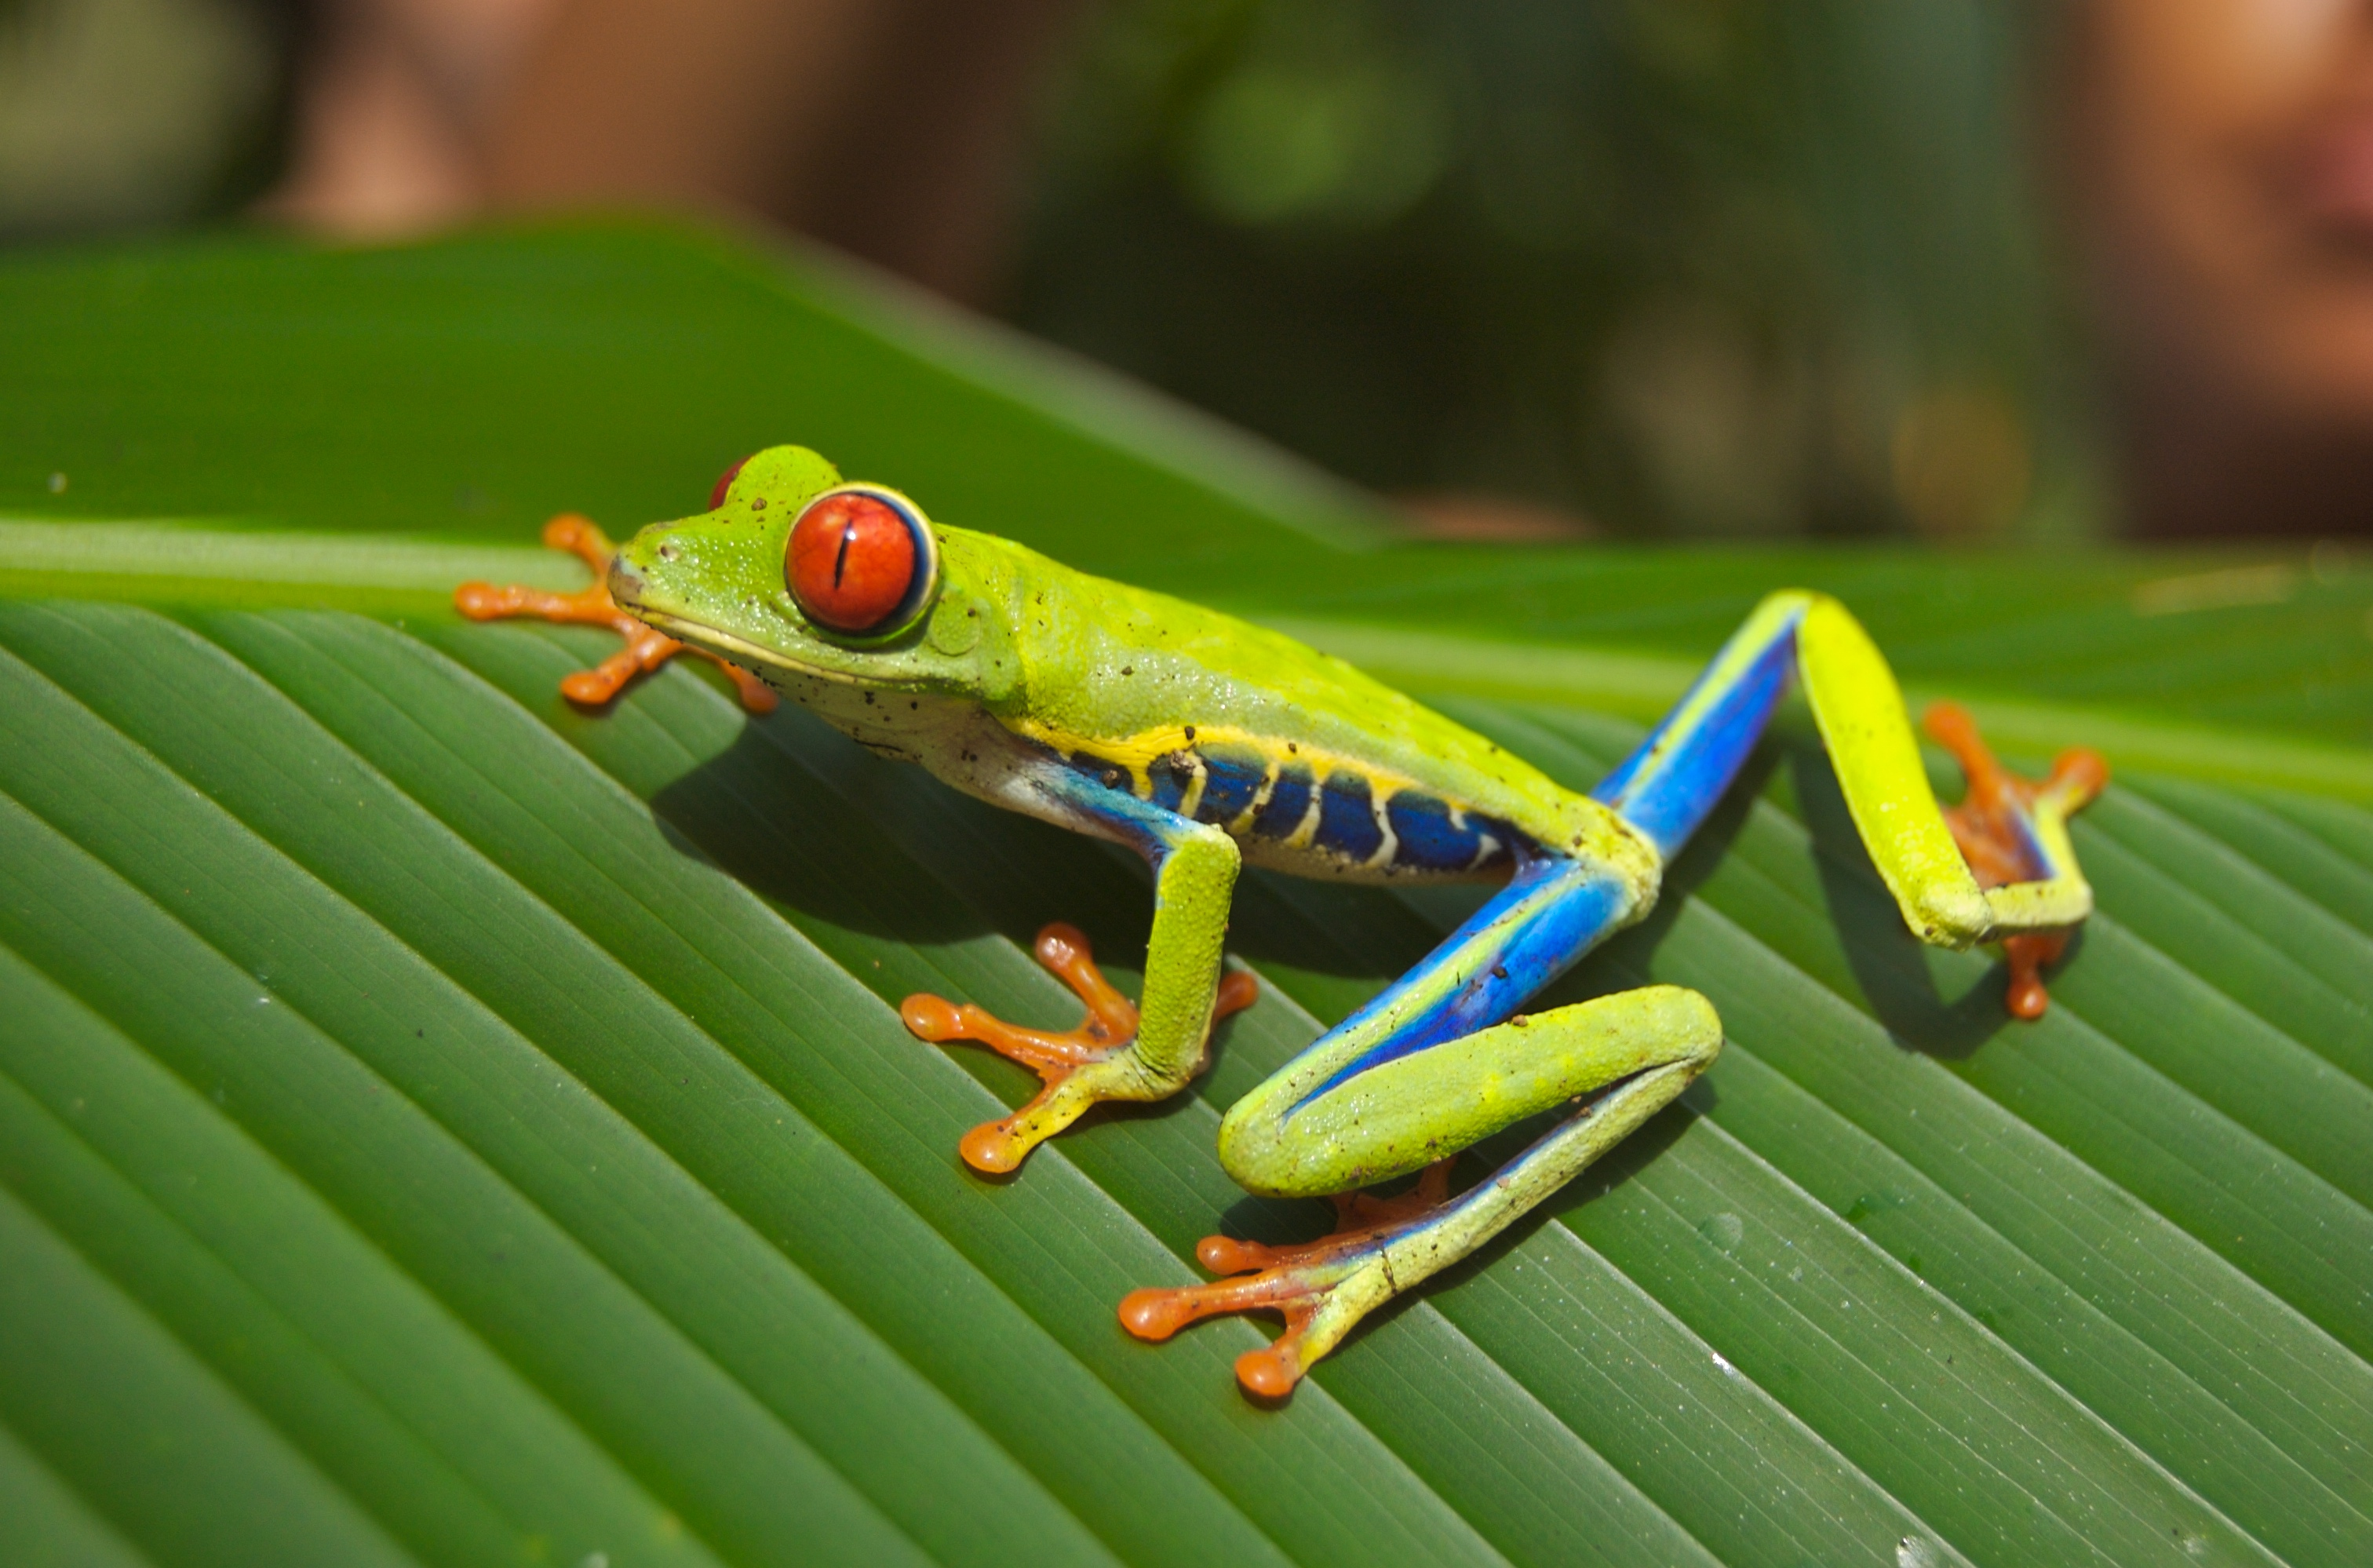
\includegraphics[width=\linewidth]{2010-lahg-09-Red_eyed_tree_frog}
	\vspace{-4ex}
\end{wrapfigure}
Väike puukonn suudab ronida mööda seinu ja lagesid, luues enda ja seina vahele 
seinaga risti oleva tõmbejõu (nt iminappade tekitatud vaakumiga) ning vältides libisemist 
selle tagajärjel tekkiva hõõrdejõu abil.
Millise nurga all maapinna suhtes peab olema sein, et tal oleks end kõige raskem paigal hoida 
(mil libisemise vältimiseks vajalik seinaga risti olev jõud on maksimaalne)?
Hõõrdetegur seina ja konna vahel on $\mu$.
\fi


\ifHint
Konnale mõjub kolm jõudu: raskusjõud, rõhumisjõu ja hõõrdejõu resultant ning putuka tekitatud tõmbejõud. Rõhumisjõu ja hõõrdejõu resultandi nurk pinnanormaali suhtes on kriitilisel juhul $\arctan \mu$. Tasakaalu korral peavad antud jõud üksteist ära tasakaalustama, ehk moodustuma kolmnurga.
\fi


\ifSolution
\begin{wrapfigure}{r}{0.5\textwidth}
	\vspace{-4ex}
	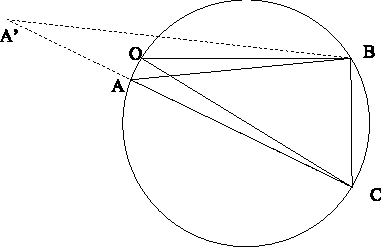
\includegraphics[width=65mm]{2010-lahg-09-lah}
	\vspace{-6ex}
\end{wrapfigure}
Konnale mõjub kolm jõudu: raskusjõud $m\vec g = \vec {BC}$, mis on suunatud vertikaalselt alla, jõud $\vec F =\vec {CA^\prime}$, 
mis on suunatud kaldpinna pinnanormaali sihis (pinna sisse)
ning rõhumisjõu ja hõõrdejõu resultant $\vec {A^\prime B}$, mille nurk pinnanormaaliga $\alpha=\angle CA^\prime B$ ei ületa väärtust 
$\arctan \mu$. Need kolm vektorit moodustavad tasakaalu korral
joonisel toodud kolmnurga $A^\prime BC$. Jooniselt on ilmne, et antud kaldenurga 
($A^\prime C$ sihi) puhul saab konn minimeerida vajalikku jõudu (st lõigu $A^\prime C$ pikkust) 
suurendades nurga $\alpha$ maksimaalse võimaliku väärtuseni $\alpha = \arctan \mu$ (mil $A^\prime = A$). Kui nüüd muuta pinna kaldenurka, 
siis joonistab punkt $A$ ringjoone kaare (sest punktid $B$ ja $C$ on fikseeritud ning $\angle BAC$ on konstantne ($\arctan \mu$). 
Vajalik jõud (lõik $AC$) on maksimaalne, kui lõik $AC$ on ringi diameetriks $OC$, st pinnanormaal moodustab horsiondiga 
nurga $\arctan\mu$ (sest $\angle OBC=90^\circ$). Seega, sein on vertikaali suhtes kaldus $\arctan \mu$ võrra, moodustades põrandaga teravnurga.

\vspace{0.5\baselineskip}

{\em Alternatiivne lahendus}\\ 
Olgu putuka tekitatud tõmbejõud $F$, hõõrdejõud $F_h$ ja normaaljõud $N$. Jõudude tasakaalu tingimusest saame
$F_{h}=mg\sin\theta$ ja $F=N+mg\cos\theta$. Kui putukas rakendab minimaalset tarvilikku jõudu, siis 

$$F_{h}=\mu N=mg\sin\theta,$$

ehk

$$N=\frac{mg\sin\theta}{\mu}.$$

Niisiis,

$$F=N+mg\cos\theta=\frac{mg\sin\theta}{\mu}+mg\cos\theta=mg\left( \frac{\sin\theta}{\mu}+\cos\theta\right).$$

Nüüd on vaja leida, millise $\theta$ korral on $F$ maksimaalne. Selleks katsume siinuse ja koosinuse summa avaldada ühe siinusena. 

Otsime A ja B nii, et kehtiks võrdus 
\[
A\sin (\theta+B)=\frac{\sin\theta}{\mu}+\cos\theta.
\]
Kuna 
\[
A\sin (\theta+B)=A\sin\theta\cos B + A\sin B \cos\theta,
\]
siis 
$A\sin B=1$ ja $A\cos B=\frac{1}{\mu}$. Siit saame $\tan B=\mu$ ja 
\[
A=\sqrt{\frac{1}{{\mu}^2} + 1}=\frac{1}{\mu}\sqrt{1+{\mu}^2}.
\]
Seega 
\[
F=\frac{mg}{\mu}\sqrt{1+{\mu}^2}\sin(\theta + \arctan\mu).
\]
Siinuse suurim võimalik väärtus on $\sin(\SI{90}{\degree})=1$, ehk $\theta + \arctan\mu=\SI{90}{\degree}$. Seega on otsitav nurk $\theta = \SI{90}{\degree}-\arctan\mu$.
\fi
}